% !TEX root = ./document.tex

\documentclass[11pt]{article}

\usepackage{mystyle}
\usepackage{myvars}

%-----------------------------

\begin{document}

  \maketitle

  %-----------------------------
  %	TEXT
  %-----------------------------


  \section{Descripción del conjunto de datos}
  \label{sec:description}

    \paragraph{}
    El conjunto de datos sobre el cual se va a realizar el análisis de la varianza se refiere a una serie de mediciones sobre el número de pulgones por planta de trigo. El experimento fue realizado recogiendo $40$ plantas (muestras aleatorias que supondremos independientes) de trigo, durante un periodo de $6$ semanas.

    \paragraph{}
    Para la realización de este análisis se ha utilizado la plataforma SAS \cite{sas}, en concreto la \emph{University Edition}. En este caso, el conjunto de datos ha sido suministrado en forma de fragmento de código, el cual se incluye en la figura \ref{code:sas_1}. El conjunto de datos sigue una estructura tabular de $240$ filas (referidas a cada observación) y $3$ columnas (referidas a la \texttt{semana}, identificador de \texttt{muestra} en esa semana y \texttt{recuento} de pulgones en dicha observación) tal y como se muestra en la figura \ref{img:pulgones-print}. El código \emph{SAS} utilizado en este caso se muestra en la figura \ref{code:sas_2}.

    \begin{figure}[!h]
      \centering
      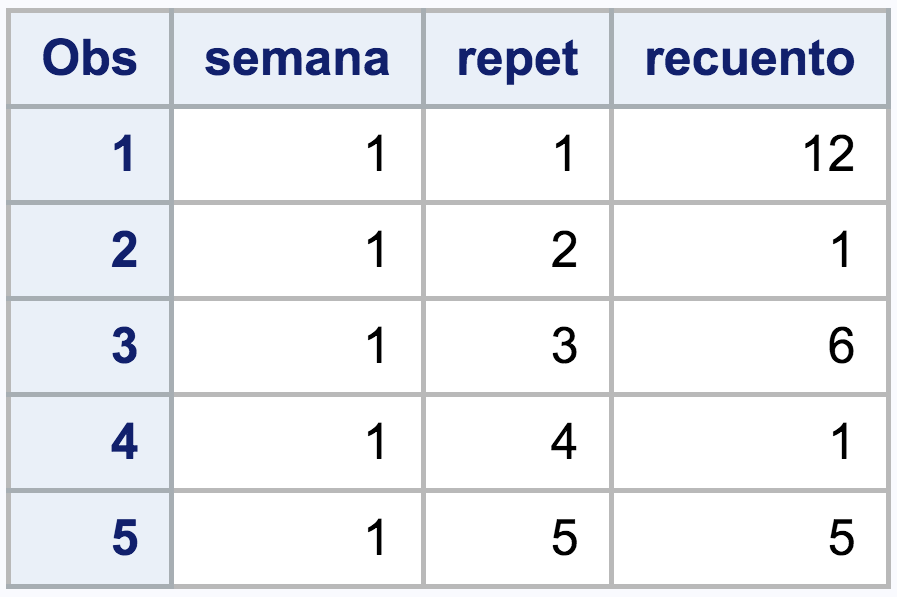
\includegraphics[width=.3\textwidth]{pulgones-print}
      \caption{Visión preliminar del conjunto de datos \texttt{pulgones}}
      \label{img:pulgones-print}
    \end{figure}

  \section{Cuestiones}
  \label{sec:questions}

    \paragraph{}
    El objetivo general del estudio es el siguiente: \textbf{\say{Se trata de analizar si existen diferencias en el número de pulgones por planta entre las diferentes semanas}}, para lo cual se proponen una seria de sub-objetivos que se tratarán de responder en las siguientes secciones.

    \subsection{?`Es adecuado utilizar un modelo de un factor para ello? Haz un análisis descriptivo de los datos por semanas y valora las hipótesis que se asumen en el modelo.}
    \label{sec:e1}

      \paragraph{}
      Para poder responder a la pregunta sobre si es adecuado utilizar un modelo de un factor para la comparación del número de pulgones por planta entre las distintas semananas, es necesario plantearse cómo han sido recogidas las observaciones, así como estudiar la distribución de la variable respuesta (\texttt{recuento} en este caso)

      \paragraph{}
      En el primer caso, se presupone que las $40$ observaciones referidas a cada semana han sido elegidas siguiendo algún procedimiento aleatorio. Por tanto, asumiremos como válida la hipótesis de independencia de las observaciones para la realización del análisis de un factor.

      \paragraph{}
      En cuanto a la hipótesis de normalidad, es decir, el estudio acerca de que los valores de la variable recuento siguen  una distribución aproximadamente normal, se ha realizado un estudio descriptivo sobre los mismos. Para dicha tarea se ha utilizado el fragmento de código incluido en la figura \ref{code:sas_3}. A partir de esta sentencia se han obtenido los resultados mostrados en la tabla de las figuras \ref{fig:normality-1}, \ref{fig:normality-2}, \ref{fig:normality-3}, \ref{fig:normality-4}, \ref{fig:normality-5} y \ref{fig:normality-6}, así como los \emph{Histogramas} incluidos en las figuras \ref{fig:histogram-plot-1-2}, \ref{fig:histogram-plot-3-4} y \ref{fig:histogram-plot-5-6} y los \emph{Gráficos de Normalidad} incluidos en las figuras \ref{fig:normal-plot-1-2}, \ref{fig:normal-plot-3-4} y \ref{fig:normal-plot-5-6}.

      \paragraph{}
      Tras el análisis de los mismos podemos empezar a sospechar acerca de una cierta falta de normalidad en los datos, concretamente en los referidos a las de la categoria \texttt{semana} $2$ y $3$. Esto se ve reflejado en los distintos valores de los tests de normalidad, así como en la apariencia de los histogramas y la marcada desviación respecto de la recta de la distirbución normal en los diagramas de \emph{cuantil-cuantil} respecto de la normal

      \begin{figure}[!h]
        \centering
        \begin{minipage}{.49\textwidth}
          \centering
          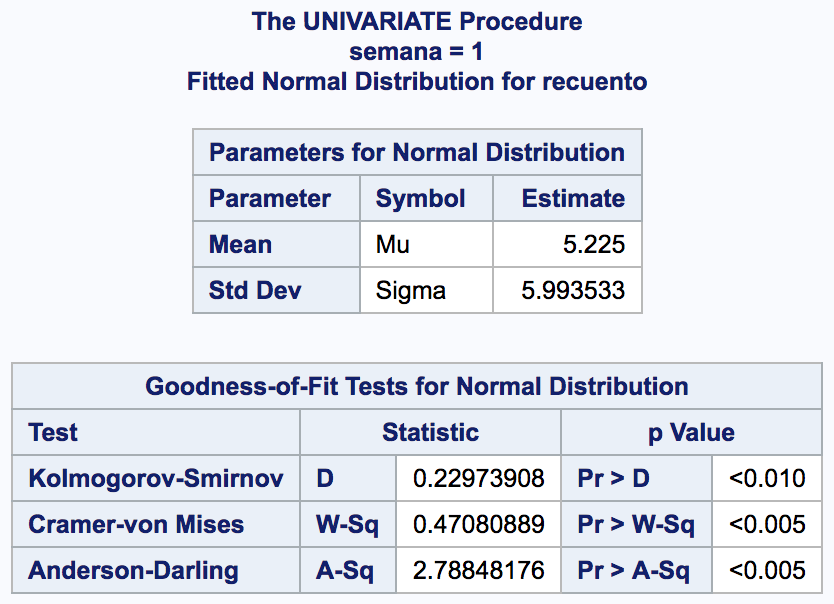
\includegraphics[width=\linewidth]{normality-1}
          \caption{}
          \label{fig:normality-1}
        \end{minipage}
        \begin{minipage}{.49\textwidth}
          \centering
          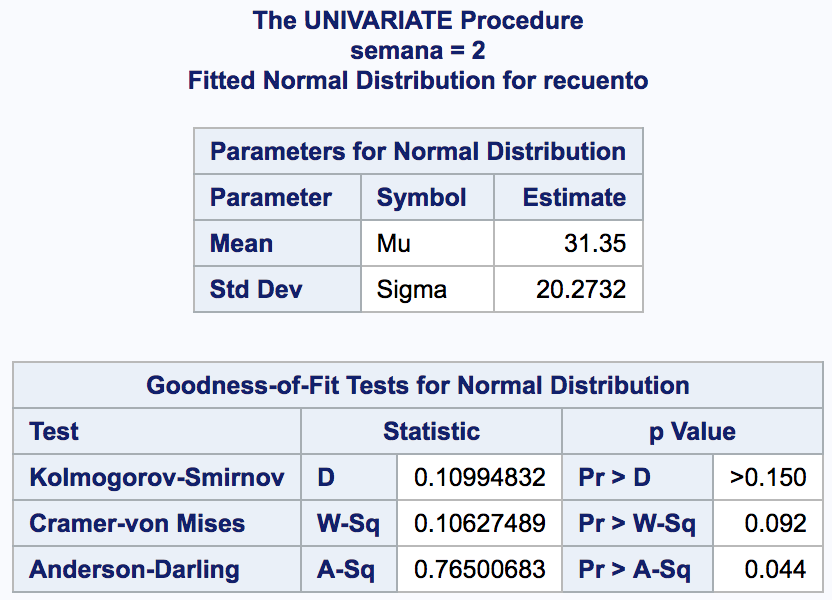
\includegraphics[width=\linewidth]{normality-2}
          \caption{}
          \label{fig:normality-2}
        \end{minipage}
        \begin{minipage}{.49\textwidth}
          \centering
          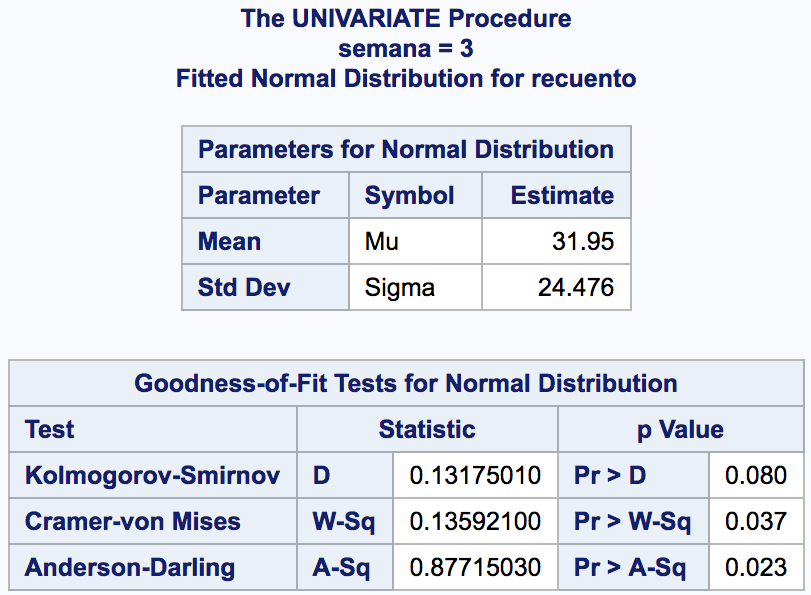
\includegraphics[width=\linewidth]{normality-3}
          \caption{}
          \label{fig:normality-3}
        \end{minipage}
        \begin{minipage}{.49\textwidth}
          \centering
          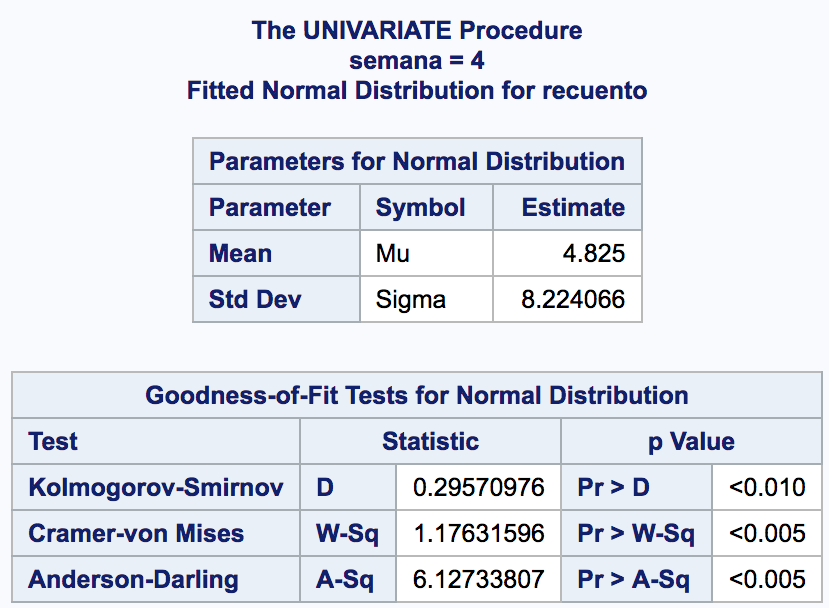
\includegraphics[width=\linewidth]{normality-4}
          \caption{}
          \label{fig:normality-4}
        \end{minipage}
        \begin{minipage}{.49\textwidth}
          \centering
          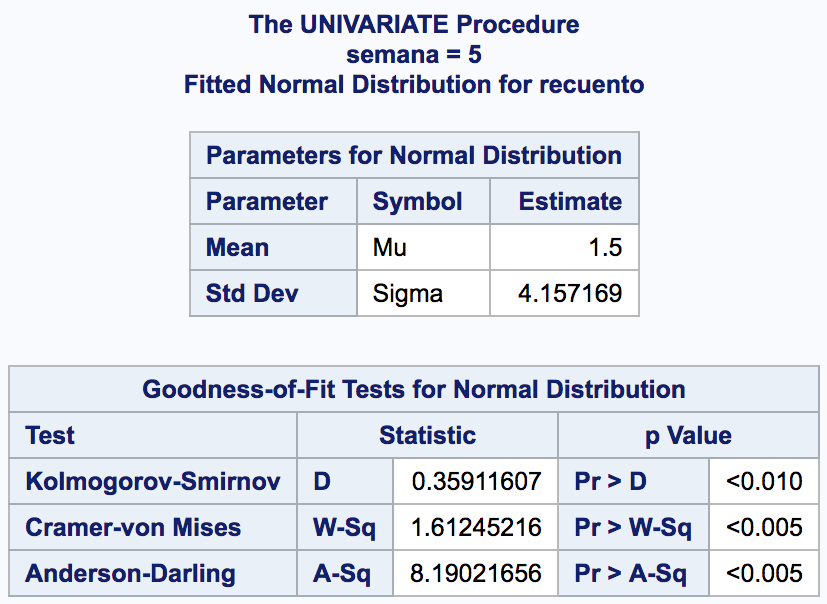
\includegraphics[width=\linewidth]{normality-5}
          \caption{}
          \label{fig:normality-5}
        \end{minipage}
        \begin{minipage}{.49\textwidth}
          \centering
          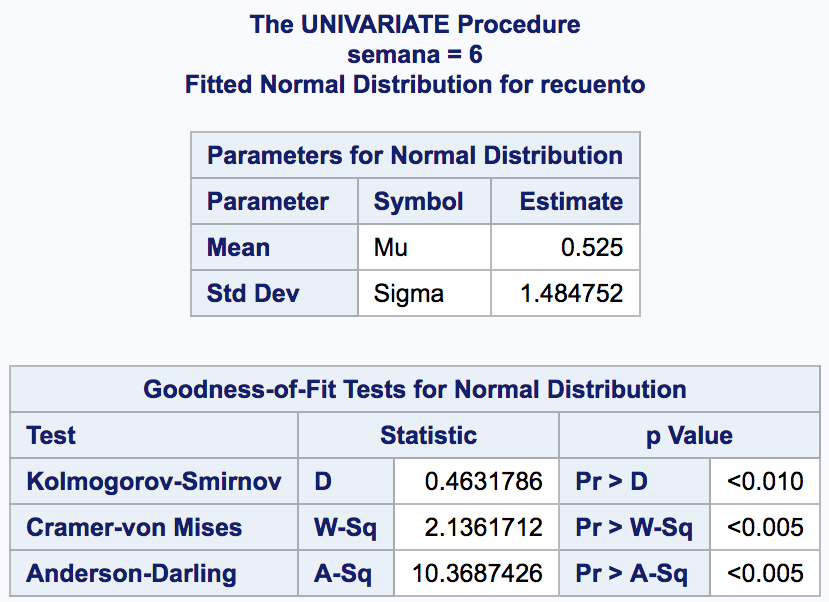
\includegraphics[width=\linewidth]{normality-6}
          \caption{}
          \label{fig:normality-6}
        \end{minipage}
      \end{figure}

      \begin{figure}[!h]
        \centering
        \begin{minipage}{.49\textwidth}
          \centering
          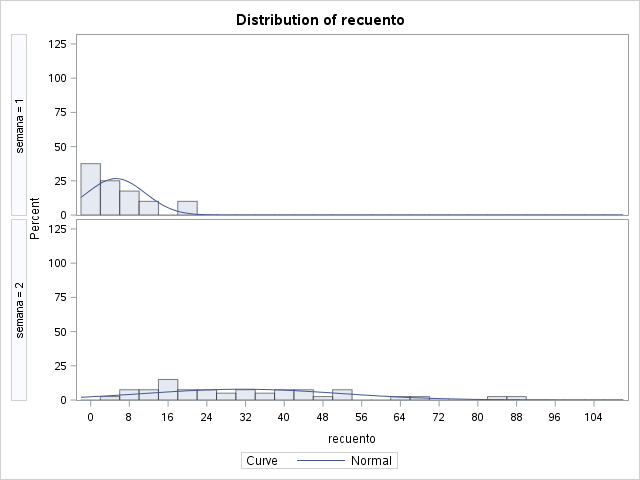
\includegraphics[width=\linewidth]{histogram-plot-1-2}
          \caption{Histograma: Semanas 1 y 2}
          \label{fig:histogram-plot-1-2}
        \end{minipage}
        \begin{minipage}{.49\textwidth}
          \centering
          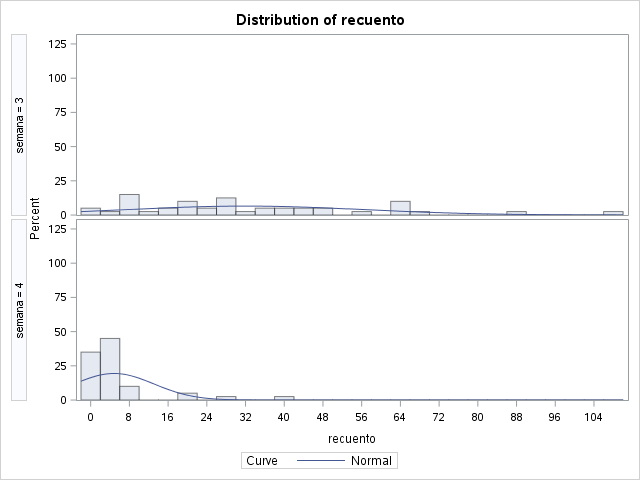
\includegraphics[width=\linewidth]{histogram-plot-3-4}
          \caption{Histograma: Semanas 3 y 4}
          \label{fig:histogram-plot-3-4}
        \end{minipage}
        \begin{minipage}{.49\textwidth}
          \centering
          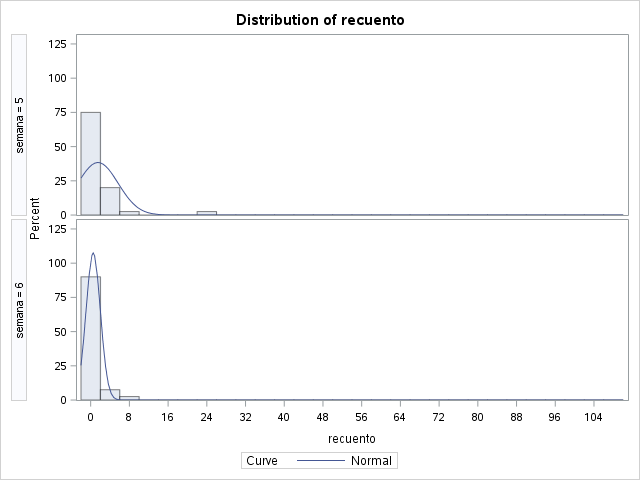
\includegraphics[width=\linewidth]{histogram-plot-5-6}
          \caption{Histograma: Semanas 5 y 6}
          \label{fig:histogram-plot-5-6}
        \end{minipage}
      \end{figure}

      \begin{figure}[!h]
        \centering
        \begin{minipage}{.49\textwidth}
          \centering
          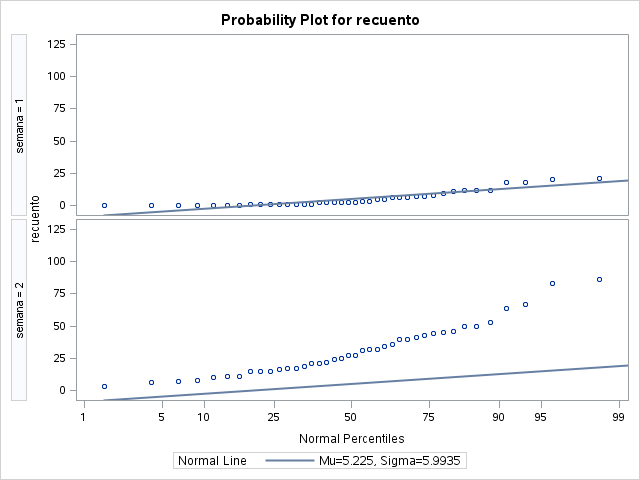
\includegraphics[width=\linewidth]{normal-plot-1-2}
          \caption{Gráfico de Normalidad: Semanas 1 y 2}
          \label{fig:normal-plot-1-2}
        \end{minipage}
        \begin{minipage}{.49\textwidth}
          \centering
          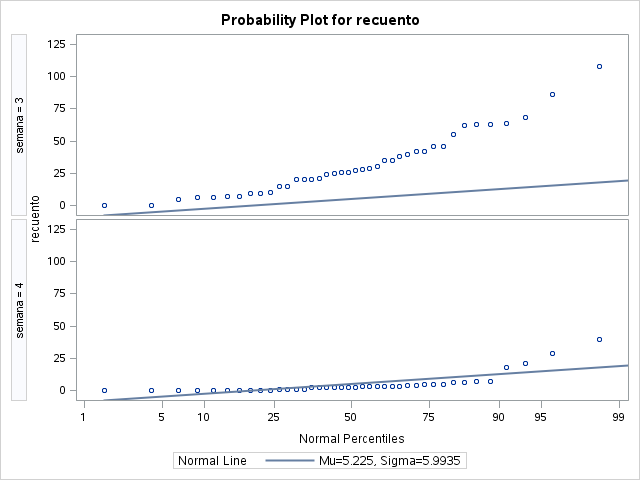
\includegraphics[width=\linewidth]{normal-plot-3-4}
          \caption{Gráfico de Normalidad: Semanas 3 y 4}
          \label{fig:normal-plot-3-4}
        \end{minipage}
        \begin{minipage}{.49\textwidth}
          \centering
          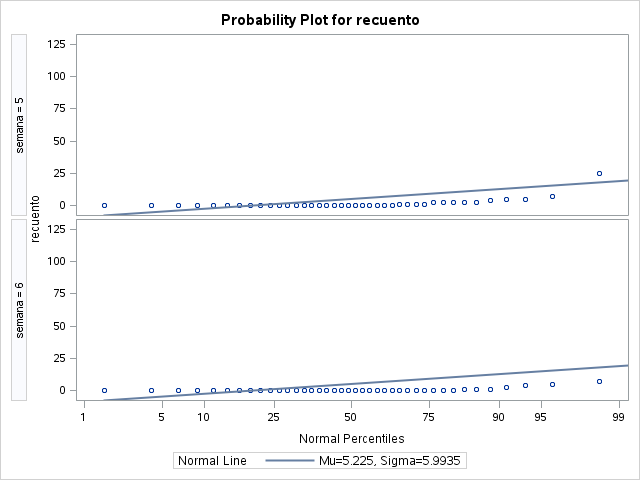
\includegraphics[width=\linewidth]{normal-plot-5-6}
          \caption{Gráfico de Normalidad: Semanas 5 y 6}
          \label{fig:normal-plot-5-6}
        \end{minipage}
      \end{figure}

      \paragraph{}
      A continuación, se ha realizado un \emph{box-plot} de la variable \texttt{recuento} divida en las categorías marcadas por \texttt{semana}, la cual se puede apreciar en la figura \ref{img:box-plot}. En este caso, se puede apreciar una clara diferencia entre las medias de las semanas 2 y 3 con respecto del resto, lo cual también sucede a nivel de la varianza.

      \begin{figure}
        \centering
        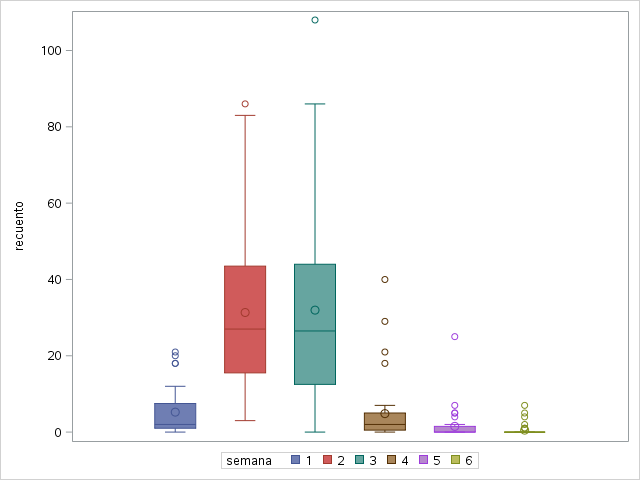
\includegraphics[width=.7\textwidth]{box-plot}
        \caption{\emph{Box-plot}: de la variable \texttt{recuento} clasificada por \texttt{semana}}
        \label{img:box-plot}
      \end{figure}

      \paragraph{}
      Por tanto, se ve reforzada la idea comentada anteriormente de falta de normalidad en el conjunto de datos. Esto hace que los contrastes de hipótesis acerca de la igualdad de medias (que asumen una distribución de varianzas igual para todos los factores) se vea gravemente comprometida. Esto hace que los resultados que se obtengan en futuras secciones tengan que ser tomados con gran prudencia.

      \paragraph{}
      Otro suceso a remarcar es el carácter temporal de los datos, que a pesar de no estar siendo estudiado en este trabajo, podría tener una alta influencia en los resultados, ya el particionamiento en categorías se está llevando a cabo sobre un soporte temporal (\texttt{semana}). Sin embargo, la descripción del conjunto de datos no especifica que estas hayan quedado descritas de una manera secuencial, es decir, no se ha determinado que existe un orden fijado por el valor de \texttt{semana}. Por tanto, es necesario tomar conclusiones prudentes en este sentido.

    \subsection{Realiza el contraste de igualdad de medias y analiza los residuos. ?`Qué conclusiones sacas?}
    \label{sec:e2}

      \paragraph{}
      Para la realización de un contraste de hipótesis referido a la igualdad de medias, se ha decidido utilizar el fragmento de código incluido en la figura \ref{code:sas_5}. Este fragmento de código realiza un contraste de igualdad de medias, y además suministra una serie de gráficos relacionados con los residuos generados por el contraste. Esto es equivalente a lo descrito en la siguiente ecuación:

      \begin{align*}
        H_0:& \quad \forall i,j \quad \mu_{i} = \mu_{j} & \\
        H_1:& \quad \exists i,j \quad \mu_{i} \neq \mu_{j} & \\
        & & i,j \in \{semana_1,...,semana_6\} \land i \neq j
      \end{align*}

      \begin{figure}[!h]
        \centering
        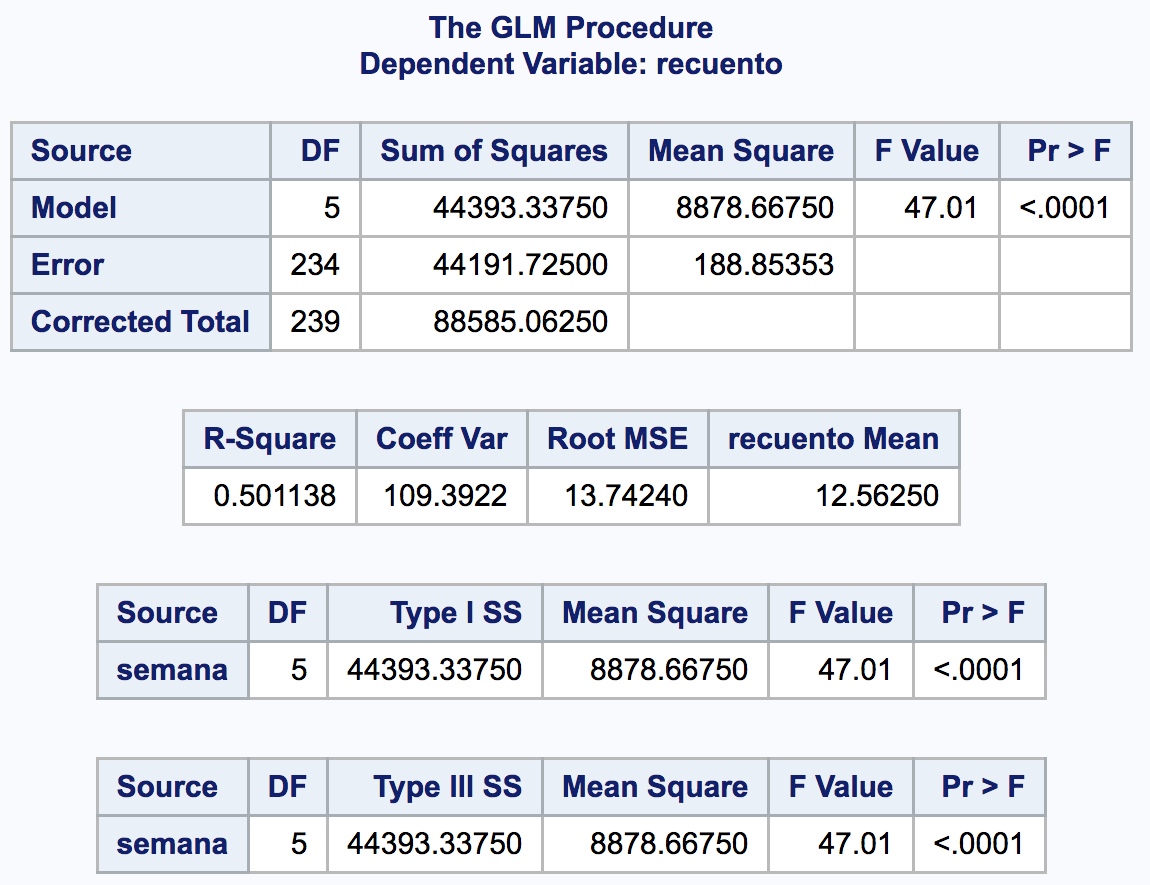
\includegraphics[width=.4\textwidth]{anova-recuento}
        \caption{Gráfico de Normalidad: Residuos del contraste de hipótesis de igualdad de medias}
        \label{img:anova-recuento}
      \end{figure}

      \paragraph{}
      El contrate de igualdad de medias ha generado los resultados obtenidos en la figura \ref{img:anova-recuento}, que tal y como se puede apreciar a partir del resultado del \emph{p-valor}, la hipótesis nula (de igualdad de medias) es rechazada con una confianza del $95\%$. Un paso intuitivo en este paso es realizar algún test múltiple como \emph{Bonferroni} o \emph{Tukey}.

      \paragraph{}
      Sin embargo, en este caso tras examinar los gráficos de residuos nos damos cuenta de que la hipótesis de igualdad de medias podría haber sido rechazada debido a la falta de normalidad de los datos. Esto se puede apreciar a través de los gráficos de residuos y residuos Studentizados de las figuras \ref{fig:scatter-plot-residuals} y \ref{fig:scatter-plot-studentized-residuals}. En los estos se aprecia la falta de normalidad, ya que los errores (en ambos casos) están claramente sesgados hacia valores positivos (algo que no debería ocurrir). En el caso de los residuos studentizados, estos superan el valor $2$ en un gran número de casos, algo que no debería ocurrir en bajo la presunción de normalidad de residuos. Otro fenómeno que se puede apreciar en estos datos es la existencia de heterocedasticidad entre las distintas categorías, que surge entre las semanas $\{ 1, 4, 5, 6\}$ y las semanas $\{ 2, 3\}$.

      \begin{figure}[!h]
        \centering
        \begin{minipage}{.49\textwidth}
          \centering
          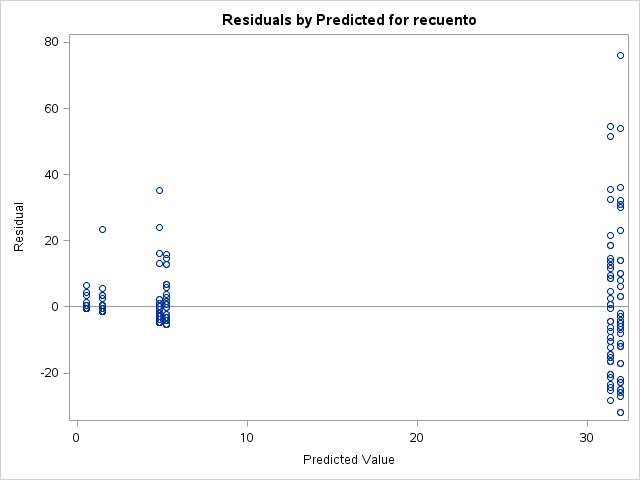
\includegraphics[width=\linewidth]{residuals}
          \caption{Scatter Plot: Residuos del contraste de hipótesis de igualdad de medias}
          \label{fig:scatter-plot-residuals}
        \end{minipage}
        \begin{minipage}{.49\textwidth}
          \centering
          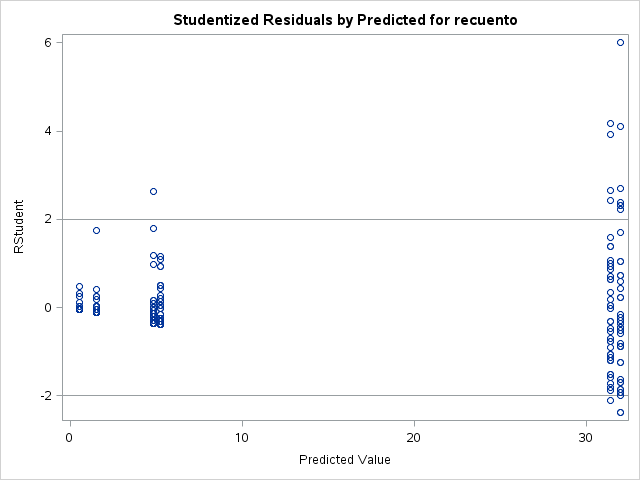
\includegraphics[width=\linewidth]{studentized-residuals}
          \caption{Scatter Plot: Residuos Studentizados del contraste de hipótesis de igualdad de medias}
          \label{fig:scatter-plot-studentized-residuals}
        \end{minipage}
      \end{figure}

      \paragraph{}
      Para confirmar la falta de normalidad en los residuos, se puede visualizar el gráfico \emph{cuantil-cuantil} de normalidad que se muestra en la figura \ref{img:normal-plot-residuals}. En este se puede apreciar una distribución que una vez más hace pensar en la inexistencia de normalidad.

      \begin{figure}[!h]
        \centering
        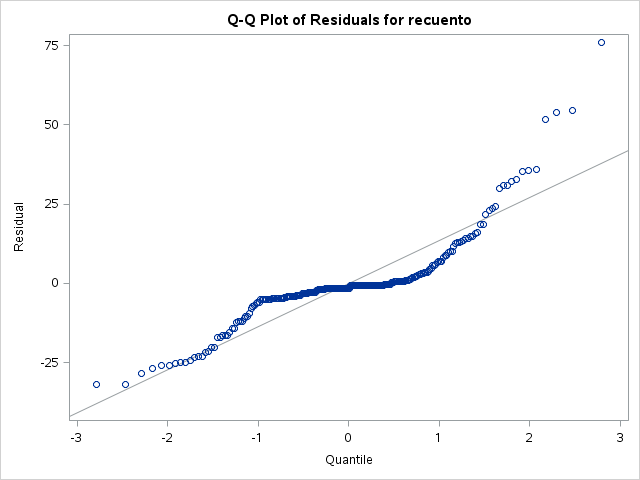
\includegraphics[width=.7\textwidth]{normal-plot-residuals}
        \caption{Gráfico de Normalidad: Residuos del contraste de hipótesis de igualdad de medias}
        \label{img:normal-plot-residuals}
      \end{figure}

    \subsection{Realiza el test de \emph{Levene}. ?`Te sorprende el resultado?}
    \label{sec:e3}

      \paragraph{}
      El código utilizado para la realización del test de \emph{Levene} se muestra en la figura \ref{code:sas_6}. Este test se refiere a la realización del contrate de hipótesis de igualdad de varianzas entre distintas poblaciones. Por tanto, se puede modelizar como:

      \begin{align*}
        H_0:& \quad \forall i,j \quad \sigma^2_{i} = \sigma^2_{j} & \\
        H_1:& \quad \exists i,j \quad \sigma^2_{i} \neq \sigma^2_{j} & \\
        & & i,j \in \{semana_1,...,semana_6\} \land i \neq j
      \end{align*}

      \paragraph{}
      Los resultados obtenidos se muestran en la figura \ref{img:levene-test}. Tras el valores, se puede apreciar que debido al reducido valor que toma el \emph{p-valor}, tenemos que rechazar la hipótesis de igualdad de varianzas con una confianza del $95\%$.

      \begin{figure}[!h]
        \centering
        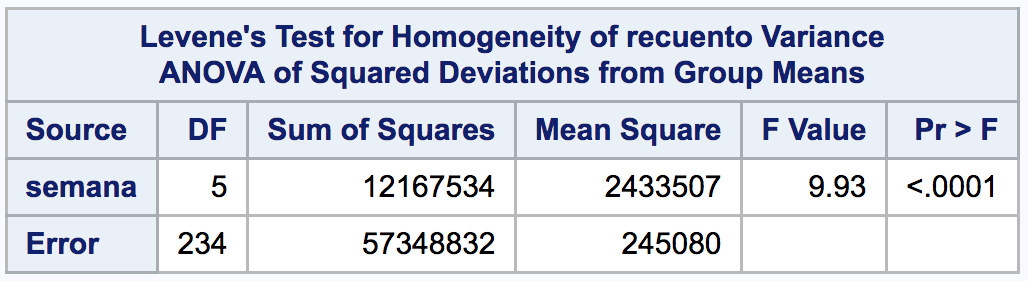
\includegraphics[width=.4\textwidth]{levene-recuento.png}
        \caption{Resultados del test de Levene de la variable \texttt{recuento} particionada por \texttt{semana}}
        \label{img:levene-test}
      \end{figure}

      \paragraph{}
      Estos resultados no sorprenden debido a las conclusiones que se habían obtenido previamente, tanto a partir de los residuos, como del \emph{box-plot} de la figura \ref{img:box-plot}, que se realizó al principio del estudio para la obtención de una visión global de los datos. A partir de estos se podía intuir la falta de igualdad de varianzas, que tras el test de \emph{Levene} se ha demostrado de manera analítica.


    \subsection{Transforma la respuesta mediante $log(recuento + 1)$ y repite el apartado \ref{sec:e2}. ?`Qué cambios observas?}
    \label{sec:e4}

      \paragraph{}
      [TODO ]


    \subsection{Realiza el test de \emph{kruskal-Wallis} sobre los datos originales para contrastar la igualdad de medias}
    \label{sec:e5}
      \paragraph{}
      [TODO ]

  \section{Código fuente}
  \label{sec:code}

    \begin{figure}[!h]
      \centering
      \begin{minted}[frame=single,framesep=5pt]{sas}
data pulgones;
  do semana=1 to 6;
    do repet=1 to 40;
      input recuento @@;
      output;
    end;
  end;
  datalines;
  12 1 6 1 5 7 1 1 2 1 20 0 9 7 0 12 2 0 0 2 8 0 11 2 21 0 3 18 2 2 6 6
  5 1 12 0 3 1 1 18 40 16 32 15 44 41 43 53 67 21 6 31 15 11 21 40 15 50
  17 32 24 7 25 11 64 22 50 27 3 46 45 10 8 27 34 19 86 83 17 36 86 63
  20 68 55 42 24 29 20 27 26 63 40 46 7 15 10 30 46 26 15 42 6 28 7 9 5
  35 6 9 108 38 35 64 21 20 62 25 0 0 29 2 3 0 4 2 6 7 5 4 6 0 0 5 1 3 2
  2 2 5 0 1 1 0 3 1 2 0 3 3 18 7 21 0 0 0 2 3 0 40 5 7 0 0 0 1 1 2 1 0
  25 1 0 0 0 0 0 0 0 5 0 2 0 0 0 2 0 0 0 4 0 0 0 0 2 0 0 0 0 2 1 0 0 1 7
  0 0 0 4 1 5 2 0 0 0 0 0 0 0 0 0 0 0 0 0 0 0 0 0 0 0 0 0 0 0 0 0 0 0 0
;
run;
      \end{minted}
      \caption{\emph{Código SAS:} Lectura del conjunto de datos.}
      \label{code:sas_1}
    \end{figure}


    \begin{figure}[!h]
      \centering
      \begin{minted}[frame=single,framesep=5pt]{sas}
proc print data=pulgones (obs=5) n;
run;
      \end{minted}
      \caption{\emph{Código SAS:} Vista preliminar del conjunto de datos.}
      \label{code:sas_2}
    \end{figure}

    \begin{figure}[!h]
      \centering
      \begin{minted}[frame=single,framesep=5pt]{sas}
proc univariate data=pulgones;
   class semana;
   var recuento;
   probplot recuento / normal
                     (mu=est sigma=est color=blue w=1);
run;
      \end{minted}
      \caption{\emph{Código SAS:} Estudio Descriptivo de la variable \texttt{recuento} particionada por \texttt{semana}.}
      \label{code:sas_3}
    \end{figure}

    \begin{figure}[!h]
      \centering
      \begin{minted}[frame=single,framesep=5pt]{sas}
proc sgplot data=pulgones;
  vbox recuento /  group=semana;
run;
      \end{minted}
      \caption{\emph{Código SAS:} \emph{Box-Plot} de la variable \texttt{recuento} particionada por \texttt{semana}.}
      \label{code:sas_4}
    \end{figure}

    \begin{figure}[!h]
      \centering
      \begin{minted}[frame=single,framesep=5pt]{sas}
proc glm data=pulgones PLOTS(UNPACK)=DIAGNOSTICS;
  class semana;
  model recuento=semana;
run;
      \end{minted}
      \caption{\emph{Código SAS:} Contraste de hipótesis de medias (con obtención de gráficos referidos a residuos).}
      \label{code:sas_5}
    \end{figure}

    \begin{figure}[!h]
      \centering
      \begin{minted}[frame=single,framesep=5pt]{sas}
proc glm data=pulgones;
  class semana;
  model recuento=semana;
  means semana / hovtest=levene;
run;
      \end{minted}
      \caption{\emph{Código SAS:} Test de \emph{Levene}}
      \label{code:sas_6}
    \end{figure}

    %-----------------------------
    %	Bibliographic references
    %-----------------------------

    \nocite{rano2017}

    \bibliographystyle{acm}
    \bibliography{bib}

\end{document}
